\documentclass[a4paper]{article}
\usepackage[utf8]{inputenc}


%=-=-=-=-=-=-=-=-=-=-=-=-=-=-=-=-=-=-=-=-=-=-=-=-=-=-=-=-=-=-=-=-=-=-=-=-=-=-=-=-
% PREAMBLE
%=-=-=-=-=-=-=-=-=-=-=-=-=-=-=-=-=-=-=-=-=-=-=-=-=-=-=-=-=-=-=-=-=-=-=-=-=-=-=-=-

%%%%%%%%%%%%%%%%%%%%%%%%%%%%%%%%%%%%%%%%%%%%%%%%%%%%%%%%%%%%%%%%%%%%%
% Important styling notes
%%
% For now, to include img.jpg in img/path/to/img.jpg, just use:
% path/to/img.jpg - for details see style.tex
%=-=-=-=-=-=-=-=-=-=-=-=-=-=-=-=-=-=-=-=-=-=-=-=-=-=-=-=-=-=-=-=-=-=-=-=-=-=-=-=-
% Packages
%%
%\usepackage{fullpage} % Package to use full page
\usepackage[top=1in,bottom=1in,left=1in,right=0.7in,heightrounded]{geometry}

\usepackage{parskip}                    % Package to tweak paragraph skipping
\usepackage{amsmath}                    % standard
\usepackage{amssymb}                    % standard - Double R symbol etc.
\usepackage{hyperref}
\usepackage{amsthm}                     % standard - theorem, definition, etc.
\usepackage{multicol}                   % multiple columns for numbering
\usepackage{enumitem}                   % standard - enumerate styles
\usepackage[utf8]{inputenc}
\usepackage{scrextend}                  % indentation
\usepackage{graphicx}                   % standard - add figures
\usepackage{float}                      % standard - figure position, use [H] option
\usepackage{pifont}                     % symbols
\usepackage{gensymb}                    % degree symbol \degree
\usepackage{xcolor}                     % bg color
\hypersetup{
    colorlinks,
    linkcolor={black!50!black},
    citecolor={blue!50!black},
    urlcolor={blue!80!black}
}
\usepackage{framed}                     % bg color
\usepackage[T1]{fontenc}                % small caps
\usepackage{sectsty}                    % headings colour
\usepackage{mathtools}                  % Loads amsmath
\usepackage{amsthm,thmtools,xcolor}     % coloured theorem
\usepackage[toc,page]{appendix}         % reference to appendix
%\usepackage{titlesec}                   % change chapter, section, etc. formats
\usepackage{xifthen}                    % if, else
\usepackage{etoolbox}
% format numbering in theorem, lemma, etc. environment
\AtBeginEnvironment{theorem}{\setlist[enumerate, 1]{font=\upshape,  wide=0.5em, before=\leavevmode}}
\AtBeginEnvironment{lemma}{\setlist[enumerate, 1]{font=\upshape,  wide=0.5em, before=\leavevmode}}
\usepackage[letterspace=150]{microtype} % \textls{<letterspaced text>} % 0 <= letterspace <= 1000, 1000 = M space
\usepackage{letltxmacro}                % renew commands?
\usepackage{minted}                     % package to list code
    % otherwise minted goes off the page
    \setmintedinline{breaklines}
\usepackage{subfig}
\usepackage{eso-pic}                    % title page bg pic
\usepackage{varwidth}
\PassOptionsToPackage{svgnames}{xcolor}
\usepackage{fontawesome}                % \faQuestionCircle
\usepackage{marvosym}                   %\Pointinghand
\usepackage{mdframed}                   % easy outline frames
\usepackage[many]{tcolorbox}            % colour box for theorem styles
\usepackage{array,booktabs,calc} % table figs and text
\usepackage{comment}                    % \begin{comment}
\usepackage{fancyhdr}                   % page headings
\usepackage{mdframed}                   % boxes
\usepackage[backend=biber,sorting=none,style=ieee]{biblatex}
\usepackage{caption}
%%% caption options {
%\DeclareCaptionFont{white}{\color{white}}
\DeclareCaptionFormat{listing}{\colorbox{magenta!30!gray}{\parbox{\textwidth}{#1#2#3}}}
\captionsetup[lstlisting]{format=listing,labelfont={bf,small},textfont=small,skip=-1pt}
%%% }
\addbibresource{bibliography.bib}
\usepackage{url}
\usepackage{textcomp}
\usepackage[makeroom]{cancel}            % crossed symbols
\usepackage{algorithm}
\usepackage[noend]{algpseudocode}
\usepackage{tikz}
\usetikzlibrary{arrows.meta,positioning,quotes} % arrows and nodes in tikz
\usepackage{marginnote}
\usepackage{pgfplots}
\usepackage{pstricks-add,pst-slpe}  % for fancy tikz arrows
%\usepackage{titlesec}                   % title style
\usepackage{lmodern}                    % a font
\usepackage{titletoc} % Required for manipulating the table of contents
\usepackage{titlesec} % Allows customization of titles
\usepackage{fouriernc} % Use the New Century Schoolbook font
\usepackage{booktabs} % things in page margins
\usepackage{stmaryrd } % \varoast
\usepackage{listings} % code listings
\usepackage{longtable} % table across multiple pages
\usepackage{styles/nasm/lang}  % include custom language for NASM assembly.
\usepackage{styles/nasm/style} % include custom style for NASM assembly.



%% extra comments that I don't know where they belong:
% list of ding tags: http://willbenton.com/wb-images/pifont.pdf

%=-=-=-=-=-=-=-=-=-=-=-=-=-=-=-=-=-=-=-=-=-=-=-=-=-=-=-=-=-=-=-=-=-=-=-=-=-=-=-=-
% Colours for various things
%%


\definecolor{shadecolor}{rgb}{1.,0.933,0.96} % bg color, r,g,b <= 1
\definecolor{medium_blue}{RGB}{60,125,190}
\definecolor{dark_blue}{RGB}{25,60,85}
\definecolor{dark_red}{RGB}{77,16,16}
\definecolor{LightPink}{rgb}{0.92.,0.8,0.84} % bg color, r,g,b <= 1
\definecolor{LighterPink}{rgb}{1.,0.94,0.97} % bg color, r,g,b <= 1
\definecolor{LightestPink}{rgb}{1.,0.95,0.99} % bg color, r,g,b <= 1
\definecolor{DarkestPink}{rgb}{0.36, 0.0, 0.18}
\definecolor{DarkerPink}{rgb}{0.41, 0.0, 0.21}
\definecolor{DarkPink}{rgb}{0.55, 0.05, 0.37}
\definecolor{lightestestpink}{RGB}{255,248,252}
\definecolor{codegray}{rgb}{0.5,0.5,0.5}
\definecolor{codegrayblue}{rgb}{0.35,0.35,0.47}



%=-=-=-=-=-=-=-=-=-=-=-=-=-=-=-=-=-=-=-=-=-=-=-=-=-=-=-=-=-=-=-=-=-=-=-=-=-=-=-=-
% Define my own theorem styles
%%

% "base" styles
\declaretheoremstyle[
  headfont=\color{DarkPink}\bfseries,
  bodyfont=\itshape,
]{colored}

\declaretheoremstyle[
  headfont=\color{DarkPink}\bfseries,
  bodyfont=\normalfont,
]{colored_upright}

% theorems (corollaries, etc) themselves, inherit from my style above
% Usage:
% \begin{theorem} \end{theorem}, \begin{lemma} \end{lemma}, ...
\declaretheorem[
	numberwithin=section,
 	style=colored,
	name=\textsc{Theorem},
]{theorem}

\tcolorboxenvironment{theorem}{
  boxrule=0pt,
  boxsep=2pt,
  colback={magenta!25!white},
  colframe=DarkPink,
  enhanced jigsaw, 
  borderline west={2pt}{0pt}{DarkPink},
  sharp corners,
  before skip=5pt,
  after skip=5pt,
  breakable,
  right=0mm % for equations
}

\declaretheorem[
	numberwithin=section,
 	style=colored,
	name=\textsc{Corollary},
]{corollary}

\tcolorboxenvironment{corollary}{
  boxrule=0pt,
  boxsep=1pt,
  colback={magenta!10!white},
  colframe=DarkPink,
  enhanced jigsaw, 
  borderline west={2pt}{0pt}{DarkPink},
  sharp corners,
  before skip=5pt,
  after skip=5pt,
  breakable,
  right=0mm % for equations
}

\declaretheorem[
	numberwithin=section,
	style=colored,
	name=\textsc{Lemma},
]{lemma}

\tcolorboxenvironment{lemma}{
  boxrule=0pt,
  boxsep=1pt,
  colback={magenta!10!white},
  colframe=DarkPink,
  enhanced jigsaw, 
  borderline west={2pt}{0pt}{DarkPink},
  sharp corners,
  before skip=5pt,
  after skip=5pt,
  breakable,
  right=0mm % for equations
}

\declaretheorem[
	numberwithin=section,
	style=colored,
	name=\textsc{Definition},
]{definition}

\tcolorboxenvironment{definition}{
  boxrule=0pt,
  boxsep=1pt,
  colback={magenta!25!white},
  colframe=DarkPink,
  enhanced jigsaw, 
  borderline west={2pt}{0pt}{DarkPink},
  sharp corners,
  before skip=5pt,
  after skip=5pt,
  breakable,
  right=0mm % for equations
}

\declaretheorem[
	numberwithin=section,
  	style=colored,
  	name=\textsc{Example},
]{exmp}

\declaretheorem[
	numberwithin=section,
  	style=colored,
  	name=\textsc{Solution},
]{soln}

%%% code listings
\lstdefinestyle{code1}{
    backgroundcolor=\color{lightestestpink},   
    commentstyle=\color{codegrayblue},
    keywordstyle=\color{DarkerPink},
    numberstyle=\tiny\color{codegray},
    stringstyle=\color{black!40!cyan},
    basicstyle=\small\ttfamily,
    breakatwhitespace=false,
    breaklines=true,        
    captionpos=t,             
    keepspaces=true,        
    numbers=left,           
    numbersep=5pt,
    showspaces=false, 
    showstringspaces=false,
    showtabs=false,
    tabsize=4
}

\lstset{style=code1}

%=-=-=-=-=-=-=-=-=-=-=-=-=-=-=-=-=-=-=-=-=-=-=-=-=-=-=-=-=-=-=-=-=-=-=-=-=-=-=-=-
% Headers (size, font, colour)
%%




\makeatletter
\renewcommand{\@seccntformat}[1]{\llap{\textcolor{DarkestPink}{\csname the#1\endcsname}\hspace{1em}}}                    
\renewcommand{\section}{\@startsection{section}{1}{\z@}
{-4ex \@plus -1ex \@minus -.4ex}
{1ex \@plus.2ex }
{\normalfont\large\sffamily\bfseries\textcolor{DarkestPink}}}
\renewcommand{\subsection}{\@startsection {subsection}{2}{\z@}
{-3ex \@plus -0.1ex \@minus -.4ex}
{0.5ex \@plus.2ex }
{\normalfont\sffamily\bfseries\textcolor{DarkestPink}}}
\renewcommand{\subsubsection}{\@startsection {subsubsection}{3}{\z@}
{-2ex \@plus -0.1ex \@minus -.2ex}
{.2ex \@plus.2ex }
{\normalfont\small\sffamily\bfseries\textcolor{DarkestPink}}}                        


%=-=-=-=-=-=-=-=-=-=-=-=-=-=-=-=-=-=-=-=-=-=-=-=-=-=-=-=-=-=-=-=-=-=-=-=-=-=-=-=-
% Numberings, counters and spacings
%%
\numberwithin{equation}{section} % section number in eq/s
\setlength{\jot}{7pt} % spacing in split, gathered env/s



%% Custom examples
%% Output - Example 1,2,...
\newcounter{example}
\newenvironment{example}[1][]{\refstepcounter{example}\par\medskip
   \textbf{Example~\theexample. #1} \rmfamily}{\medskip}
%%%%%%%%%%%% End of unused %%%%%%%%%%%%



%=-=-=-=-=-=-=-=-=-=-=-=-=-=-=-=-=-=-=-=-=-=-=-=-=-=-=-=-=-=-=-=-=-=-=-=-=-=-=-=-
% Paths
%%
\graphicspath{ {./img/} } % figures' path - can look up files directly from there


%=-=-=-=-=-=-=-=-=-=-=-=-=-=-=-=-=-=-=-=-=-=-=-=-=-=-=-=-=-=-=-=-=-=-=-=-=-=-=-=-
% User defined macros (math mode)
%%


% Curly braces under text. Usage: \myunderbrace{upper}{lower}
\newcommand{\myunderbrace}[2]{\mathrlap{\underbrace{\phantom{#1}}_{#2}} #1}
\newcommand{\setR}{\mathbb{R}} % \ouble R
\newcommand{\setRn}{\mathbb{R}^n} %  double R^n
\newcommand{\setN}{\mathbb{N}} % double N
\newcommand{\setZ}{\mathbb{Z}} % double Z
\let\oldemptyset\emptyset
\let\emptyset\varnothing % nice - looking empty set symbol
\newcommand{\fancyN}{\mathcal{N}} % null space
\newcommand{\fancyR}{\mathcal{R}} % range

\newcommand{\bx}{\textbf{x}}
\newcommand{\by}{\textbf{y}}
\newcommand{\bb}{\textbf{b}}
\newcommand{\bA}{\textbf{A}}
\newcommand{\bB}{\textbf{B}}
\newcommand{\bI}{\textbf{I}}
% double bars as in norm
\newcommand{\norm}[1] {\lVert #1 \rVert} 
\newcommand{\trans}[1]{#1^{\top}}

\newcommand{\mean}[1]{\bar{#1}}
\newcommand{\var}{\sigma^2}

\newcommand{\partdevx}[1]{\frac{\partial #1}{\partial x}}
\newcommand{\partdevxx}[1]{\frac{\partial #1}{\partial x}}
\newcommand{\partdevxn}[1]{\frac{\partial^n #1}{\partial x^n}}
\newcommand{\partdevy}[1]{\frac{\partial #1}{\partial x}}
\newcommand{\partdevyy}[1]{\frac{\partial #1}{\partial y}}
\newcommand{\partdevyn}[1]{\frac{\partial^n #1}{\partial y^n}}

% text above = symbol
\newcommand{\overeq}[1]{\ensuremath{\stackrel{#1}=}} 
\newcommand{\greatersmaller}{%
  \mathrel{\ooalign{\raisebox{.6ex}{$>$}\cr\raisebox{-.6ex}{$<$}}}
} % greater and smaller symbols on top of each other, same line

%=-=-=-=-=-=-=-=-=-=-=-=-=-=-=-=-=-=-=-=-=-=-=-=-=-=-=-=-=-=-=-=-=-=-=-=-=-=-=-=-
% User defined macros (non math)

\newcommand{\qedblack}{$\hfill\blacksquare$} % black square end of line
\newcommand{\qedwhite}{\hfill \ensuremath{\Box}} % white square end of line
\newcommand{\hquad}{\hskip0.5em\relax}% half quad space
%\newcommand{\TODO}{\textcolor{red}{\bf TODO!}\;}

\newcommand{\TODO}[1][]{%
    \ifthenelse{\equal{#1}{}}{\textcolor{red}{\bf TODO!}\;}{\textcolor{red}{\textbf {TODO:} #1}\; }%
}
\newcommand{\B}[1]{\textbf{\textup{#1}}} % bold and upright
\renewcommand{\labelitemi}{\scriptsize$\textcolor{DarkPink}{\blacksquare}$} % itemize - squares instead of bullets
\newcommand{\emphasis}[1]{\textls{#1}}

\LetLtxMacro{\originaleqref}{\eqref}
\renewcommand{\eqref}{Eq.~\originaleqref}
\renewcommand*{\eqref}[1]{Eq.~\originaleqref{#1}}





% background images
%%%%%%%
\newcommand\BackgroundPic{%
\put(0,0){%
\parbox[b][\paperheight]{\paperwidth}{%
\vfill
%\centering

\includegraphics[width=0.125\paperwidth,height=\paperheight,%
]{img/background_02.png}% use ,keepaspectratio
\vfill
}}}
%%%%%%%
% end of background image
%%%%%%%%%%%%%% my own frame
\newmdenv[topline=false,bottomline=false]{leftrightbox}
%%%%%%%%%%%%% end
%%%%%%%%%%%%% my own comment
\newcommand{\mycomment}[1]{\begin{leftrightbox}\Pointinghand~\textbf{Comment:}~#1 \end{leftrightbox}}
%%%%%%%%%%%%% end
% my custom note https://tex.stackexchange.com/questions/301993/create-custom-note-environment-with-tcolorbox
\newmdenv[
    topline=false,
    bottomline=false,
    rightline=false,
    innerrightmargin=0pt
]{siderule}
\newenvironment{mynote}%
    {\begin{siderule}\textbf{\Pointinghand~Note:}}
    {\end{siderule}}
%%%%%%%%%%%%% my own box
\newcommand{\boxone}[1]{\begin{tcolorbox}[colback = LighterPink,colframe=LightPink]
#1
\end{tcolorbox}}
%%%%%%%%%%%%% end

\let\oldemptyset\emptyset
\let\emptyset\varnothing
%algorithmic
\algdef{SE}[DOWHILE]{Do}{doWhile}{\algorithmicdo}[1]{\algorithmicwhile\ #1}%



%%% from https://tex.stackexchange.com/questions/20267/how-to-construct-a-confusion-matrix-in-latex
\newcommand\MyBox[2]{
  \fbox{\lower0.75cm
    \vbox to 1.7cm{\vfil
      \hbox to 1.7cm{\hfil\parbox{1.4cm}{#1\\#2}\hfil}
      \vfil}%
  }%
}
%%%


\begin{document}
%=-=-=-=-=-=-=-=-=-=-=-=-=-=-=-=-=-=-=-=-=-=-=-=-=-=-=-=-=-=-=-=-=-=-=-=-=-=-=-=-
% GLOBAL STYLES (DOCUMENT SCOPE)
%=-=-=-=-=-=-=-=-=-=-=-=-=-=-=-=-=-=-=-=-=-=-=-=-=-=-=-=-=-=-=-=-=-=-=-=-=-=-=-=-
% caption: Figure 1 -> <bold> Fig. 1 </bold>
\captionsetup[figure]{labelfont={bf},labelformat={default},labelsep=period,name={Fig.}}


%=-=-=-=-=-=-=-=-=-=-=-=-=-=-=-=-=-=-=-=-=-=-=-=-=-=-=-=-=-=-=-=-=-=-=-=-=-=-=-=-
% TITLE PAGE
%=-=-=-=-=-=-=-=-=-=-=-=-=-=-=-=-=-=-=-=-=-=-=-=-=-=-=-=-=-=-=-=-=-=-=-=-=-=-=-=-
%%%%%%%%%%%%%%%%%%%%%%%%%%%%%%%%%%%%%%%%%
% Formal Book Title Page
% LaTeX Template
% Version 2.0 (23/7/17)
%
% This template was downloaded from:
% http://www.LaTeXTemplates.com
%
% Original author:
% Peter Wilson (herries.press@earthlink.net) with modifications by:
% Vel (vel@latextemplates.com)
%
% License:
% CC BY-NC-SA 3.0 (http://creativecommons.org/licenses/by-nc-sa/3.0/)
% 
% This template can be used in one of two ways:
%
% 1) Content can be added at the end of this file just before the \end{document}
% to use this title page as the starting point for your document.
%
% 2) Alternatively, if you already have a document which you wish to add this
% title page to, copy everything between the \begin{document} and
% \end{document} and paste it where you would like the title page in your
% document. You will then need to insert the packages and document 
% configurations into your document carefully making sure you are not loading
% the same package twice and that there are no clashes.
%
%%%%%%%%%%%%%%%%%%%%%%%%%%%%%%%%%%%%%%%%%

%----------------------------------------------------------------------------------------
%	PACKAGES AND OTHER DOCUMENT CONFIGURATIONS
%----------------------------------------------------------------------------------------



%----------------------------------------------------------------------------------------
%	TITLE PAGE
%----------------------------------------------------------------------------------------



\begin{titlepage} % Suppresses headers and footers on the title page

	\centering % Centre everything on the title page
	
	\scshape % Use small caps for all text on the title page
	
	\vspace*{\baselineskip} % White space at the top of the page
	
	%------------------------------------------------
	%	Title
	%------------------------------------------------
	
	\rule{\textwidth}{1.6pt}\vspace*{-\baselineskip}\vspace*{2pt} % Thick horizontal rule
	\rule{\textwidth}{0.4pt} % Thin horizontal rule
	
	\vspace{0.75\baselineskip} % Whitespace above the title
	
	{\LARGE COMPUTER VISION NOTES\\ \Large OBJECT LOCALISATION AND TRACKING\\} % Title
	
	\vspace{0.75\baselineskip} % Whitespace below the title
	
	\rule{\textwidth}{0.4pt}\vspace*{-\baselineskip}\vspace{3.2pt} % Thin horizontal rule
	\rule{\textwidth}{1.6pt} % Thick horizontal rule
	
	\vspace{2\baselineskip} % Whitespace after the title block
	
	%------------------------------------------------
	%	Subtitle
	%------------------------------------------------
	My personal notes on
	
	\vspace*{3\baselineskip} % Whitespace under the subtitle
	
	Object Localisation Techniques; Colour Matching, Mean Shift Tracking, Optical Flow, Lukas Kanade 
	
	\vspace*{3\baselineskip} % Whitespace under the subtitle
	
	%------------------------------------------------
	%	Editor(s)
	%------------------------------------------------
	
	By
	
	\vspace{0.5\baselineskip} % Whitespace before the editors
	
	{\normalfont \Large \mintinline{latex}{0xLeo} (\url{github.com/0xleo}) \\} % Editor list
	
	\vspace{0.5\baselineskip} % Whitespace below the editor list
	
	%\textit{The University of California \\ Berkeley} % Editor affiliation
	
	\vfill % Whitespace between editor names and publisher logo
	
	%------------------------------------------------
	%	Publisher
	%------------------------------------------------
	
	
	\vspace{0.3\baselineskip} % Whitespace under the publisher logo
	
	\today % Date
	
	{DRAFT X.YY} % Draft version
	{\\Missing: \ldots}

\end{titlepage}

%----------------------------------------------------------------------------------------

%\maketitle



%=-=-=-=-=-=-=-=-=-=-=-=-=-=-=-=-=-=-=-=-=-=-=-=-=-=-=-=-=-=-=-=-=-=-=-=-=-=-=-=-
% MAIN DOCUMENT
%=-=-=-=-=-=-=-=-=-=-=-=-=-=-=-=-=-=-=-=-=-=-=-=-=-=-=-=-=-=-=-=-=-=-=-=-=-=-=-=-
\newpage
\tableofcontents
\newpage



%------------------------------ New section ------------------------------%
\section{Meausing the quality of a binary classifier}

The problem we attempt to answer in this article is; when is a binary classifier reliable given a dataset? What's a good quality measure? From now on, we assume that the classifier can predict only two classes - \textit{positive} and \textit{negative}.

\subsection{Binary classification terms -- actual vs predicted}

We assume that we have a number of positive and negative samples as input as attempt to predict (label) them as positive or negative. Therefore we have 4 prediction cases:
\begin{enumerate}
    \item Positive input and positive prediction -- True Positive (TP). \textcolor{green!60!black}{Good}.
    \item Positive input and negative prediction -- False Negative (FN). \textcolor{red!60!black}{Bad}.
    \item Negative input and positive prediction -- False Positive (FP). \textcolor{red!60!black}{Bad}.
    \item Negative input and negative prediction -- True Negative (TN). \textcolor{green!60!black}{Good}. 
\end{enumerate}

To make it easier to understand these terms, we can visualise them in a matrix called \emphasis{confusion matrix}. It is split into four quarters.

\begin{figure}[H]
    \centering
    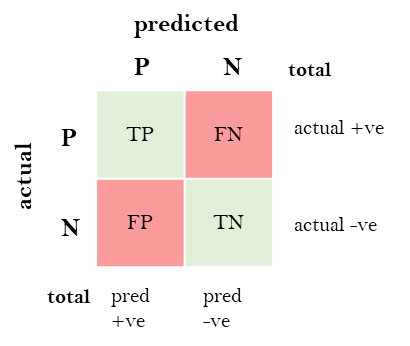
\includegraphics[height=5.5cm]{img/conf_matrix.png}
    \caption{Confusion matrix.}
\end{figure}

Ideally, a binary classifier labels all inputs 100\% correctly, therefore outputs only TP's or TN's, but of course that's not always the case. What does the number of FP and FN compared to TP and TN say about the quality of its predictions?

%\url{https://data-science-blog.com/blog/2019/03/07/a-gentle-introduction-to-precision-and-recall/}\\
%\url{https://developers.google.com/machine-learning/crash-course/classification/precision-and-recall}\\
%\url{https://towardsdatascience.com/accuracy-recall-precision-f-score-specificity-which-to-optimize-on-867d3f11124}\\
%\url{https://www.mikulskibartosz.name/precision-vs-recall-explanation/}\\
%\url{https://blog.exsilio.com/all/accuracy-precision-recall-f1-score-interpretation-of-performance-measures/}\\


\subsection{Performance metrics}

\begin{definition}[accuracy]
Accuracy is the ratio of correctly predicted samples over the total number of samples.
\begin{equation}
    Acc := \frac{TP + TN}{TP + FP + TN + FN}
\end{equation}
\end{definition}
Accuracy does not perform well with unbalanced datasets. For example, imagine we have a large image of $N$ pixels and we want to detect a face in the distance by classifying whether each pixel corresponds to the face or not. The vast majority of pixels in the image are \textit{not} face pixels (actual negatives) and a few are (actual positives). A badly-designed classifier could predict 0 face pixels. Therefore $TN \approx N, \ TP = 0,\ FP = 0,\ FN \approx 0$. Then the accuracy would falsely indicate that this is an almost perfect classifier as
\[
Acc = \frac{TP + TN}{TP + FP + TN + FN} \approx \frac{N}{N} \approx 1
\]
Precision aims to answer the question; ``What proportion of positive predictions was actually correct?''. 
\begin{definition}[Precision]
Therefore precision is defined as the ratio of TP over the total predicted positives.
\begin{equation}
    Prec = \frac{TP}{TP + FP}
\end{equation}
\end{definition}
For the face detection example, precision would be the ratio of correctly predicted face pixels compared to all pixels predicted as face. Assume a badly-designed classifier correctly detected only a few face pixels but did not falsely detect background objects as face. Therefore it would have some $TP$, lots of $TN$, some $FN$ and 0 $FP$. The precision would be perfect, although the classifier may not necessarily perform well:
\[
Prec = \frac{TP}{TP + FP} = \frac{TP}{TP + 0} = 1
\]
Precision itself is not a good metric and we don't know whether it is applied on all skin pixels or only a small sample of then -- i.e. identify all relevant instances. The measure that identifies all relevant instances is the recall (a.k.a. sensitivity). Recall attempts to answer; ``What proportion of actual positives was identified correctly?''
\begin{definition}[recall]
Therefore recall is defined as the ratio of TP over all the actuall positives ($TP + FN$):
\begin{equation}
    Rec = \frac{TP}{TP + FN}
\end{equation}
\end{definition}
Referring to the face detection example, if another bad classifier labelled all face pixels as face \textit{and} all pixels around them as such, overestimating the face pixels, then $FN = 0$ and let $TP = s$. Then the recall would be perfect, although the classifier  does not necessarily perform well:
\[
Rec = \frac{TP}{TP + FN} = \frac{s}{s + 0} = 1
\]
The latter classifier would correctly extract all relevant face pixel instances and have high recall. However it wouldn't correctly label all predicted positives, having lots of FP's, therefore low precision. 

% add face imgs (https://sanfrancisco.cbslocal.com/2015/12/06/sunnyvale-police-seek-alleged-package-thief-caught-home-surveillance-camera/)
The figures below illustrate how recall and precision alone are not always good metrics.

\begin{multicols}{3}
\begin{figure}[H]
    \centering
    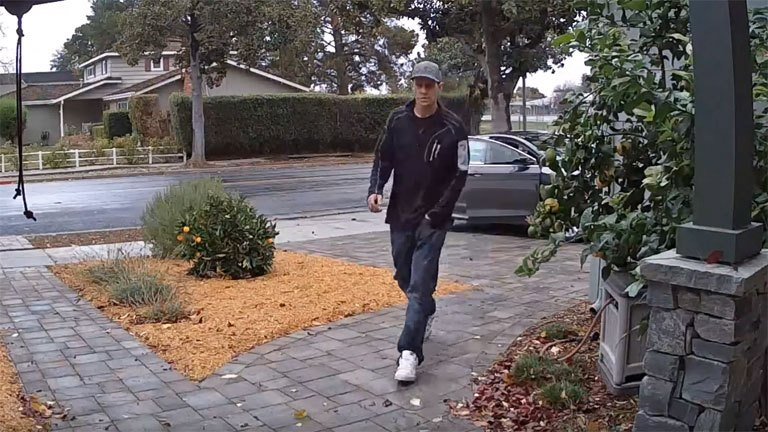
\includegraphics[width=.33\textwidth]{img/face_unmarked.jpg}
    \caption{Face pixel classifier has detected nothing at all. However, $Acc \approx 100\%$.}
\end{figure}
\columnbreak
\begin{figure}[H]
    \centering
    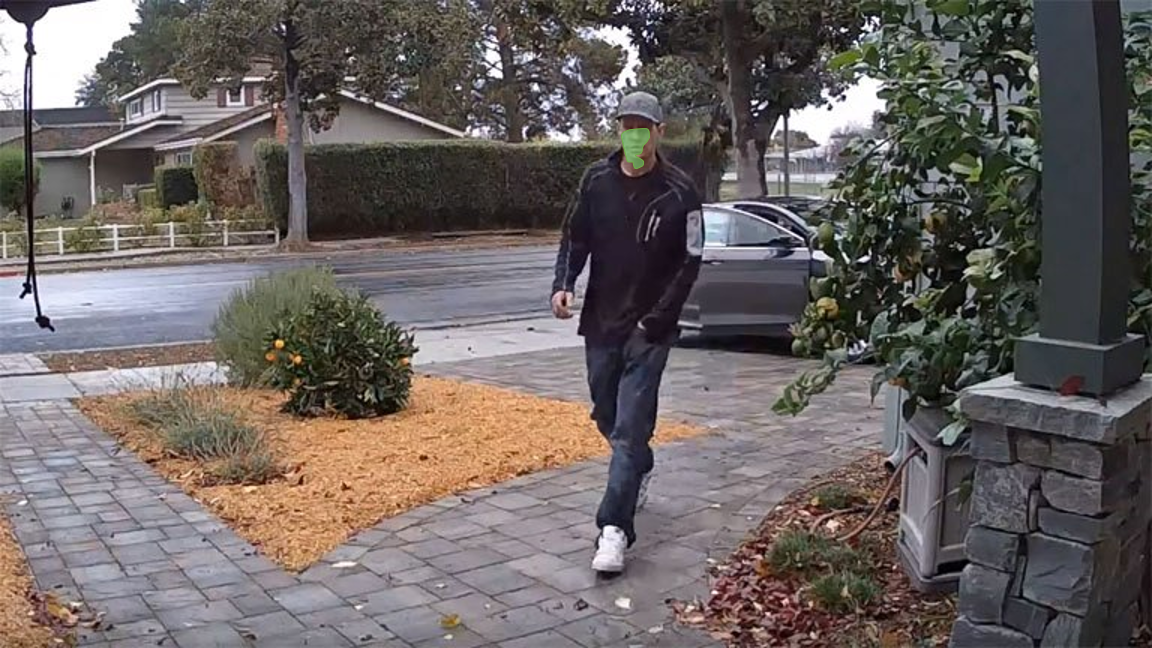
\includegraphics[width=.33\textwidth]{img/face_fn.png}
    \caption{Detected face pixels are green. Classifier has failed to mark a lot of face pixels. $FP = 0$ therefore $Prec = 100\%$ but recall is low.}
\end{figure}
\columnbreak
\begin{figure}[H]
    \centering
    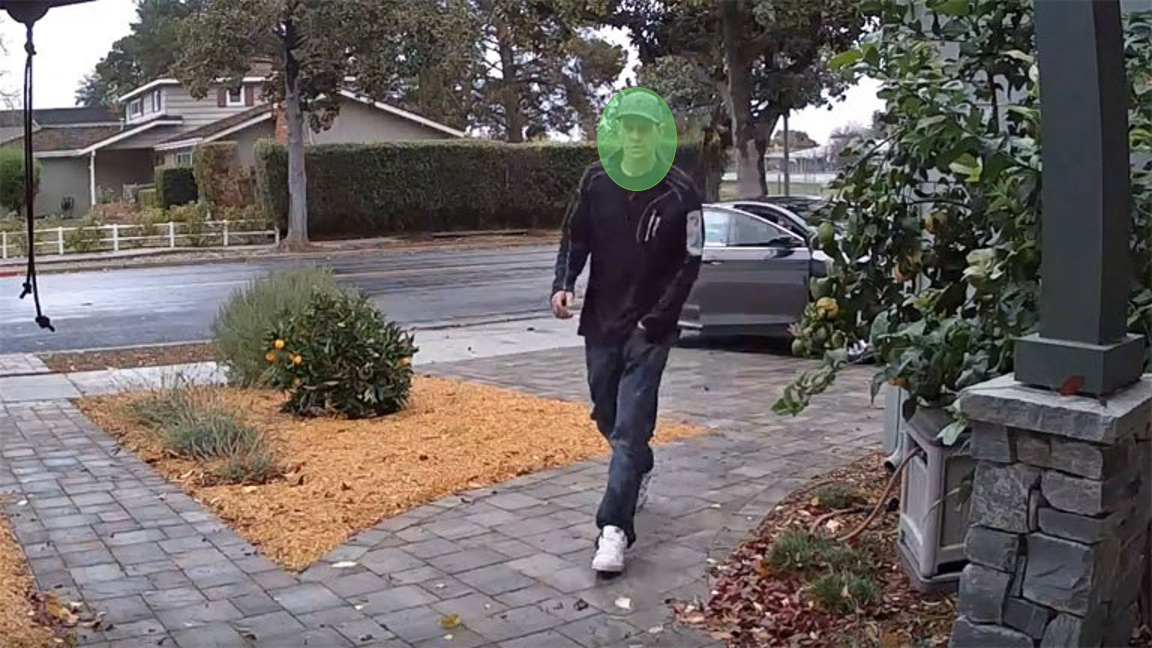
\includegraphics[width=.33\textwidth]{img/face_fp.png}
    \caption{Classifier has laballed a lot of background pixels as skin (FP). However, $FN = 0$ therefore $Rec = 100\%$ and precision is low.}
\end{figure}
\end{multicols}

% see https://towardsdatascience.com/accuracy-recall-precision-f-score-specificity-which-to-optimize-on-867d3f11124
A measure that combines both precision and recall is the $F1$ score.
\begin{definition}[f1 score]
$F1$ score is defined as the harmonic mean of precision and recall:
\begin{equation}
    F1 = \frac{2 \cdot Prec \cdot Rec}{Prec + Rec}
\end{equation}
\end{definition}
$F1$ Score is best if there is some sort of balance between precision ($p$) and recall ($r$) in the system. Oppositely, $F1$ score isn't so high if one measure is improved at the expense of the other. For example, if $p=1, \ r = 0$,\ $F1=0$.




\subsection{When is a binary classifier accurate? The ROC curve.}

% see also https://datascience.stackexchange.com/questions/31872/auc-roc-of-a-random-classifier
A binary classifier is considered good when it performs better than the random classifier. We will see how we can compare a classifier to the random one in the newxt few paragraphs. One thing to keep in mind about the random classifier is the following; let's say we have an input set with $n_p$ positive and $n_n$ negative instances. Then the actual positive probability is $p(X=1) = \frac{n_p}{n_p+n_n}$ and the actual negative is $p(X=0) = 1 - p(X=1)$. A random classifier (is random because) will randomly assign each input to the positive class with probability $\rho$ and to the negative class with probablity $1-\rho$. Therefore for the random classifiers the numbers of TP, FN, TN, FP are the combined probabilities of the class and the assignment:
\begin{align}
    TP &= \rho p(X=1) \label{eq:random_class_tp}\\
    FN &= (1-\rho)p(X=1) \label{eq:random_class_fn}\\
    TN &= (1-\rho)p(X=0) \label{eq:random_class_tn}\\
    FP &= \rho p(X=0) \label{eq:random_class_fp}
\end{align}
As shown in the following diagram, due to its nature a random classifier labels \textit{equal fraction} $\rho$ of positive instances as positive ($TP/P$) and negative instances as positive ($FP/N$).
\begin{figure}[H]
    \centering
    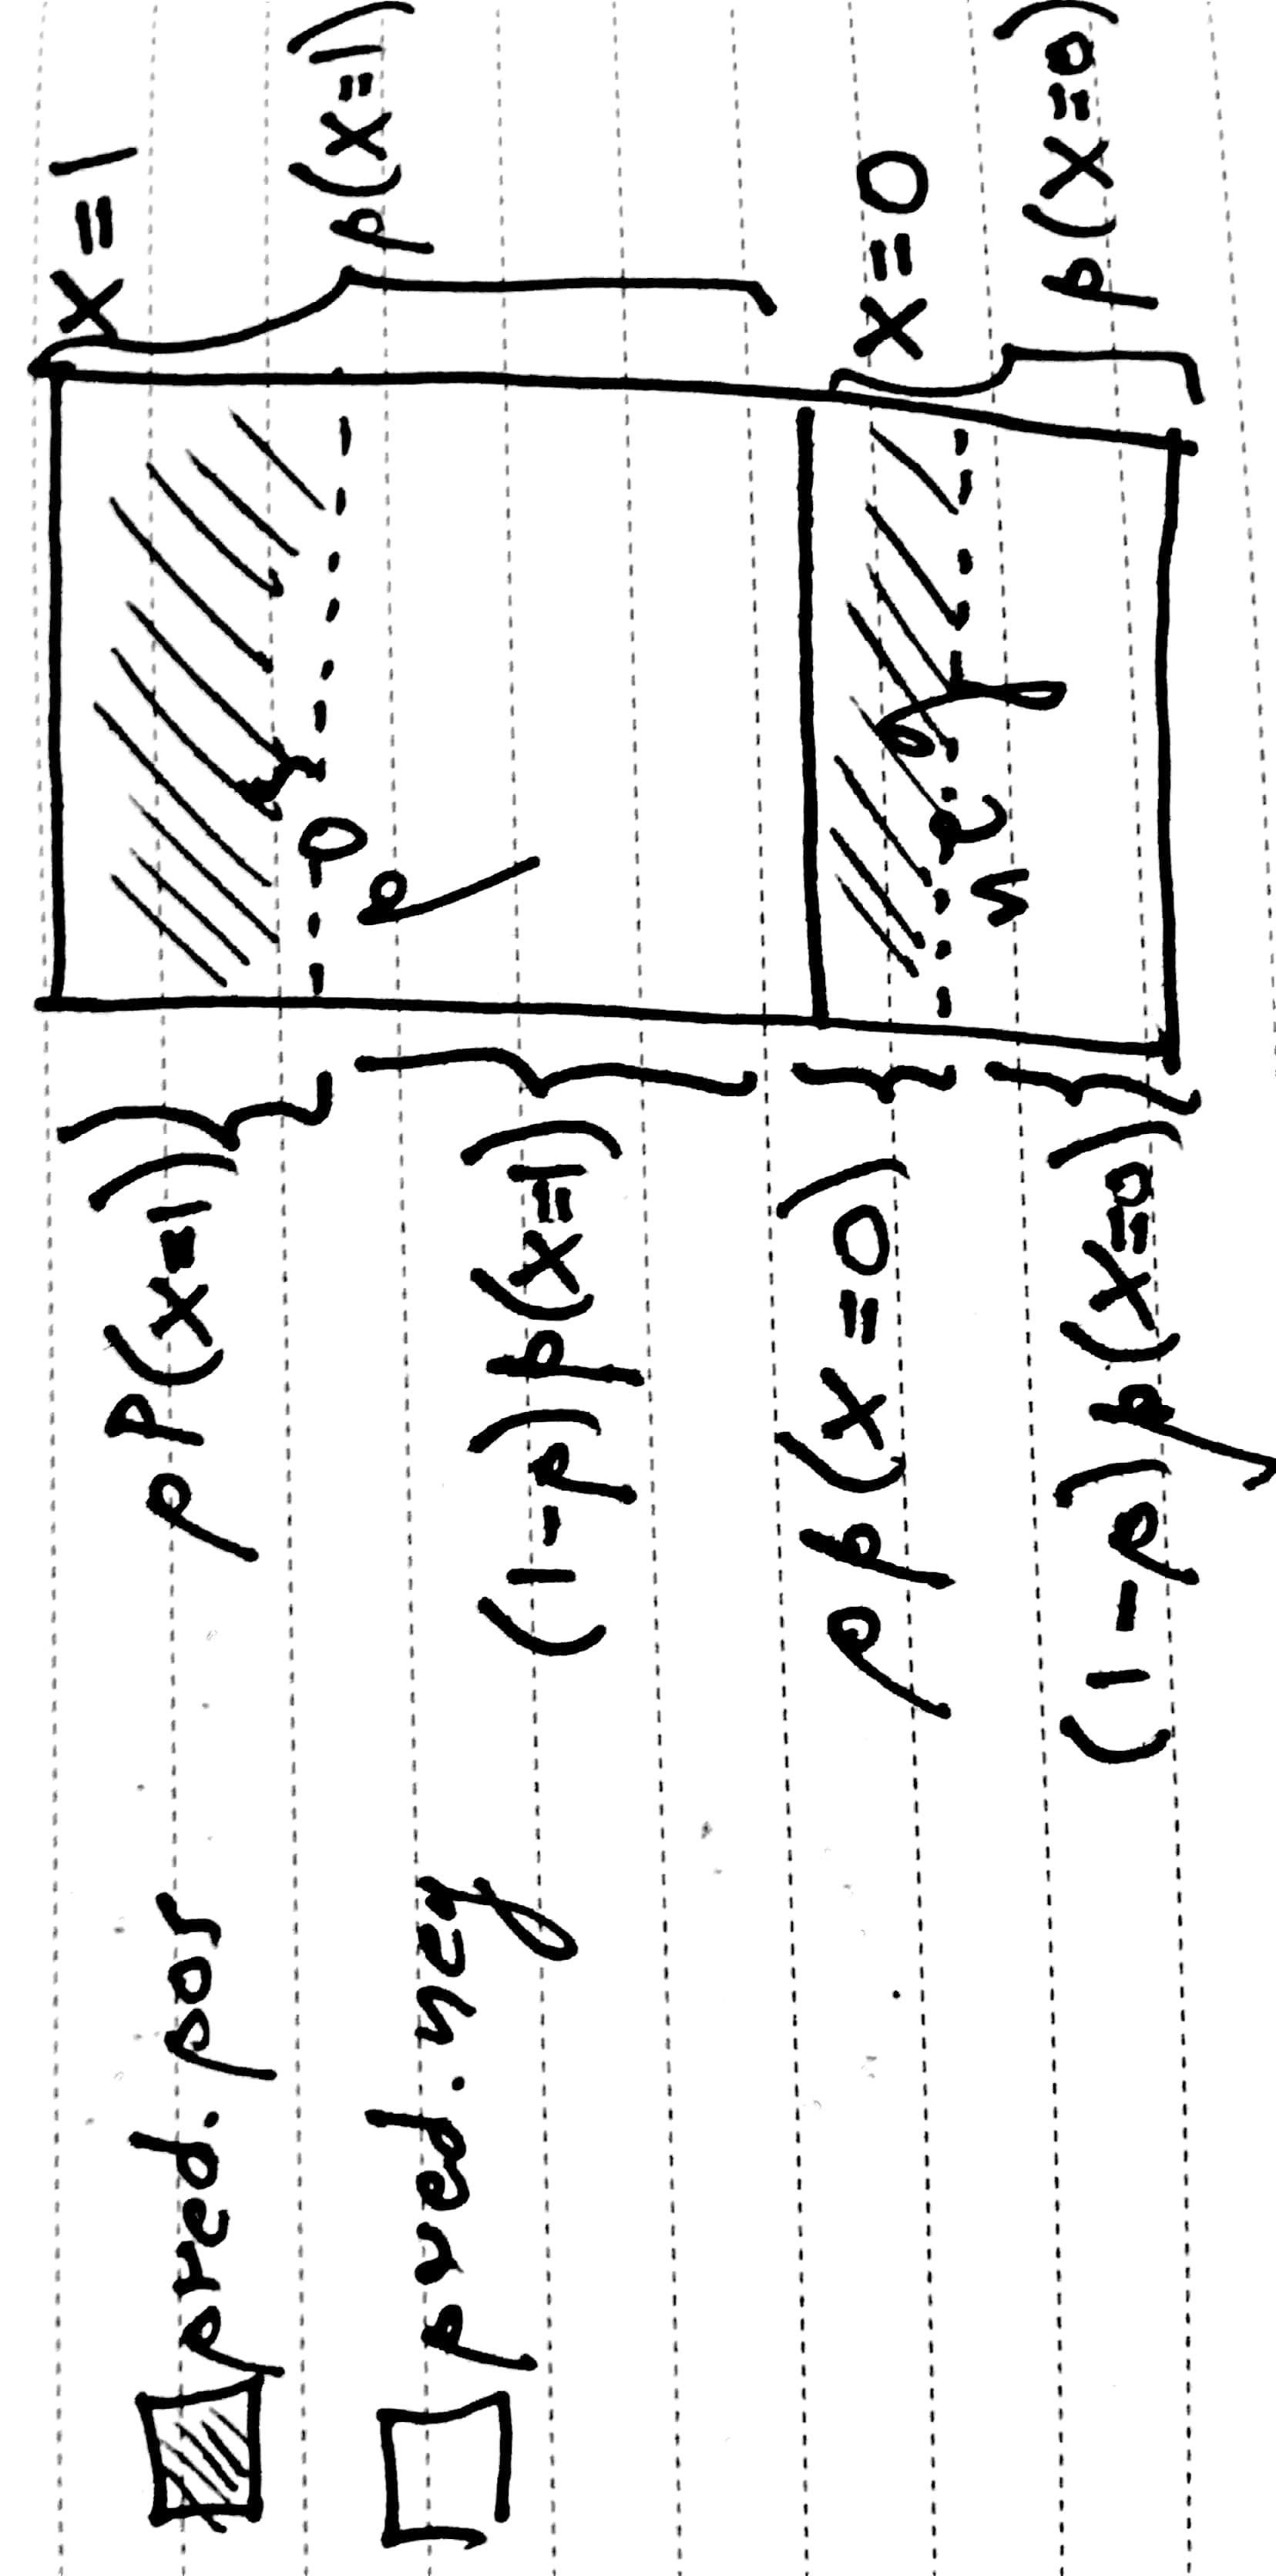
\includegraphics[scale=.07,angle=-90]{img/unbalanced_dataset.jpg}
    \caption{How the random classifier's output depends on the class balance and the current decision ($\rho$).}
    \label{fig:unlanced_datasets}
\end{figure}




\marginnote{The name comes from WWII when it was used to evaluate the performance of radars!}The tool to measure a classifier's performance is the \emphasis{Receiver Operating Characteristic (ROC) curve}. ROC curve uses some terms which we define below.

% see https://en.wikipedia.org/wiki/Receiver_operating_characteristic
\begin{definition}[sensitivity]
In ROC curve terms, recall is also called sensitivity or True Positive Rate (TPR), defined as we saw before as:
\begin{equation}
    TPR = \frac{TP}{P} = \frac{TP}{TP + FN}
\end{equation}
\end{definition}

\begin{definition}[fall-out]
False positive rate (FPR) (or fall-out) is defined as:
\begin{equation}
    FPR = \frac{FP}{N} = \frac{FP}{FP + TN}
\end{equation}
\end{definition}

% see % see https://www.medcalc.org/manual/roc-curves.php
In a ROC curve the true TPR (sensitivity) is plotted in function of the FPR for different cut-off points. Therefore to construct the whole curve we need to vary either the positive or the negative class probability in the input dataset from $P(X=1)=0$ to $P(X=1)=1$. Each point on the ROC curve represents a TPR/ FPR pair therefore a different confusion matrix instance. A test with perfect discrimination has a ROC curve that passes through the upper left corner (100\% sensitivity -- no FN, 0\% fall-out -- no FP). Therefore the closer the ROC curve is to the upper left corner, the higher the overall accuracy of the test.

As mentioned before, a classifier is good if it performs better than the random one. The figure below visualises some good and bad points in the ROC space. The ``good'' points are above the line $y=x$, which is the ROC curve of the random classifier.


%%% TODO: temp
\vspace{3cm}

\begin{multicols}{2}
\begin{figure}[H]
    \centering
    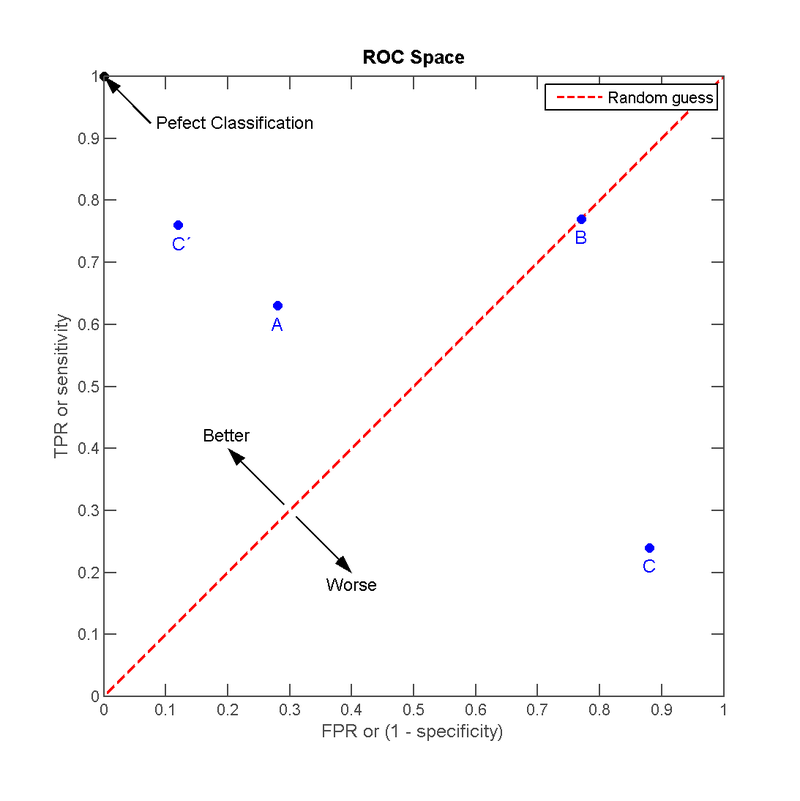
\includegraphics[height=6cm]{img/roc_space.png}
    \caption{The ROC space and plots of the four prediction examples. Source: wikepedia.}
\end{figure}
\columnbreak
\begin{figure}[H]
    % ref https://www.medcalc.org/manual/roc-curves.php
    \centering
    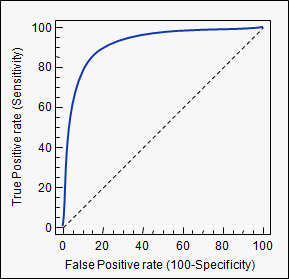
\includegraphics[height=5cm]{img/ideal_roc_curve.png}
    \caption{Ideal ROC curve. It passes near  point $(FPR,TPR)=(0,1)$}
\end{figure}
\end{multicols}

\begin{corollary}
The ROC curve (TPR over FPR) of the random classifier is the line $y=x$.
\end{corollary}
\begin{proof}
From \eqref{eq:random_class_tp} and \eqref{eq:random_class_fn}, for the TPR of a random classifier we have:
\[
TPR = \frac{TP}{TP+FN} = \frac{\rho p(X=1)}{\rho p(X=1) + (1-\rho)p(X=1)} = \rho \tag{1}
\]
From \eqref{eq:random_class_fp} and \eqref{eq:random_class_tn} for the FPR:
\[
FPR = \frac{FP}{FP+ TN} = \frac{\rho p(X=0)}{\rho p(X=0) + (1 -\rho )p(X=0)} = \rho \tag{2}
\]
Therefore $FPR = TPN = \rho \;\ \forall \ 0\leq \rho \leq 1$. This fact that these rates are both equal to $\rho$ is also intuitive from Fig. \ref{fig:unlanced_datasets}. 

\end{proof}


\subsection{Area Under ROC Curve (AUC)}

The last question is how exactly do we measure the ``quality'' of the ROC curve, especially when two curves look similar? A robust  measure we use to assess the overall performance of a binary classifier is the \emphasis{Area Under the ROC Curve (AUC)}. AUC is a robust measure as it relies on the complete ROC curve and thus involves all possible classification thresholds. It measures the area under the curve within points the box $(0,0),(1,1)$.

One way of interpreting AUC is as the probability that the model ranks a random positive example more highly than a random negative example. AUC ranges in $[0,1]$. The higher the value, the better the classifier (Fig. \ref{fig:auc_a_vs_b}). In general, AUC value in range $[0.5,1]$ are considered good as the AUC of a random classifier is $0.5$. A AUC of that range means that our binary classifier in general performs better than a random one.
\begin{figure}[H]
    \centering
    %src https://link.springer.com/referenceworkentry/10.1007%2F978-1-4419-9863-7_209
    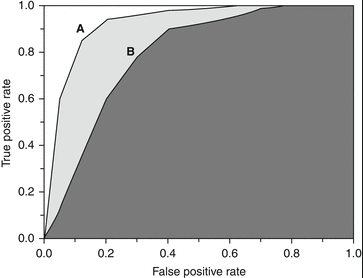
\includegraphics[height=5cm]{img/auc_of_a_vs_b.PNG}
    \caption{Binary classifier A has higher AUC so it performs better \cite{Melo2013}.}
    \label{fig:auc_a_vs_b}
\end{figure}

\begin{corollary}
A binary classifier performs well if it's AUC is higher than 0.5, where 0.5 is the AUC of a random classifier.
\end{corollary}



%\url{https://datascience.stackexchange.com/questions/31872/auc-roc-of-a-random-classifier}\\
%\url{https://www.researchgate.net/post/How_to_tell_if_an_F1-score_or_MCC_score_is_better_than_random_for_a_binary_classifier}




%\url{https://developers.google.com/machine-learning/crash-course/classification/roc-and-auc}\\
%\url{https://stats.stackexchange.com/questions/132777/what-does-auc-stand-for-and-what-is-it}\\
%\url{https://link.springer.com/referenceworkentry/10.1007%2F978-1-4419-9863-7_209}\\


%\url{https://medium.com/greyatom/lets-learn-about-auc-roc-curve-4a94b4d88152}\\
%\url{https://developers.google.com/machine-learning/crash-course/classification/roc-and-auc}\\
%\url{https://acutecaretesting.org/en/articles/precision-recall-curves-what-are-they-and-how-are-they-used}\\
%\url{https://www.datascienceblog.net/post/machine-learning/interpreting-roc-curves-auc/}\\
%\url{https://datascience.stackexchange.com/questions/31872/auc-roc-of-a-random-classifier}\\




%=-=-=-=-=-=-=-=-=-=-=-=-=-=-=-=-=-=-=-=-=-=-=-=-=-=-=-=-=-=-=-=-=-=-=-=-=-=-=-=-
% Appendices
%=-=-=-=-=-=-=-=-=-=-=-=-=-=-=-=-=-=-=-=-=-=-=-=-=-=-=-=-=-=-=-=-=-=-=-=-=-=-=-=-
%\newpage
%\appendix

%\section{Appendices}

% ------------------------ New appendix ------------------------ %
%\newpage
%\subsection{Appendix Example}
%\label{app:my_cool_appendix}


%=-=-=-=-=-=-=-=-=-=-=-=-=-=-=-=-=-=-=-=-=-=-=-=-=-=-=-=-=-=-=-=-=-=-=-=-=-=-=-=-
% References
%=-=-=-=-=-=-=-=-=-=-=-=-=-=-=-=-=-=-=-=-=-=-=-=-=-=-=-=-=-=-=-=-=-=-=-=-=-=-=-=-
\newpage
\printbibliography


\end{document}